\documentclass[12pt,a4paper,oneside]{article}
\usepackage[a4paper,left=2cm,right=1cm,top=2cm,bottom=2cm]{geometry}

\usepackage{polyglossia}
\setmainlanguage{russian}
\PolyglossiaSetup{russian}{indentfirst=true}

\usepackage{fontspec}
\defaultfontfeatures{Mapping=tex-text}

\setmainfont{Times New Roman}
\setromanfont{Times New Roman}
\setsansfont{Arial}
\setmonofont{Courier New}

\newfontfamily{\cyrillicfont}{Times New Roman}
\newfontfamily{\cyrillicfontrm}{Times New Roman}
\newfontfamily{\cyrillicfonttt}{Courier New}
\newfontfamily{\cyrillicfontsf}{Arial}

\usepackage{graphicx}
\graphicspath{{img/}}

\usepackage{float}
\floatstyle{plaintop}
\restylefloat{table}
  
\usepackage{color, listings}
\lstset{
  basicstyle=\footnotesize\ttfamily,
  inputpath=src/,
  numbers=left,
  showstringspaces=false,
  %upquote=true,
  xleftmargin=\parindent,
}
\renewcommand{\lstlistingname}{Листинг}

\begin{document}

\begin{titlepage}
    \begin{center}
      \begin{large}
        Национальный исследовательский ядерный университет <<МИФИ>> \\
        \vspace{0.25cm}
        Институт интеллектуальных кибернетических систем \\
        \vspace{0.25cm}
        Кафедра №12 <<Компьютерные системы и технологии>>
      \end{large}
  
      \vspace*{1cm}
  
      \begin{figure}[H]
        \centering
        \begin{minipage}[c]{0.3\textwidth}
          
\includegraphics[width=\textwidth]{logo_university}
        \end{minipage}
        \hfill
        \begin{minipage}[c]{0.3\textwidth}
          
\includegraphics[width=\textwidth]{logo_institute}
        \end{minipage}
        \hfill
        \begin{minipage}[c]{0.3\textwidth}
          
\includegraphics[width=\textwidth]{logo_department}
        \end{minipage}
      \end{figure}
  
      \vspace{4cm}
  
      \begin{huge}
        \textbf{ОТЧЕТ}
      \end{huge}
  
      \begin{large}
        \textbf{О выполнении лабораторной работы №1 \\
          <<Изучение принципов сложения целых чисел>>}
      \end{large}
      
      \vfill
      
      \begin{flushright}
        \begin{tabular}{ r l }
          \textbf{Cтудент:} & Почесушкин~И.\,А. \\ 
          \textbf{Группа:} & Б99-495 \\  
          \textbf{Преподаватель:} & Доцентиков~Ю.\,Б. \\
        \end{tabular}
      \end{flushright}
              
      Москва~--- 2022
    \end{center}
  \end{titlepage}

\setcounter{page}{2}

\section{Формулировка индивидуального задания}

Вариант №1. Написать программу для сложения двух целых чисел.


\section{Описание использованных типов данных}

При выполнении данной лабораторной работы использовался
встроенный тип данных \texttt{int},
предназначенный для работы с целыми числами.


\section{Описание использованного алгоритма}

\begin{figure}[H]
  \centering
  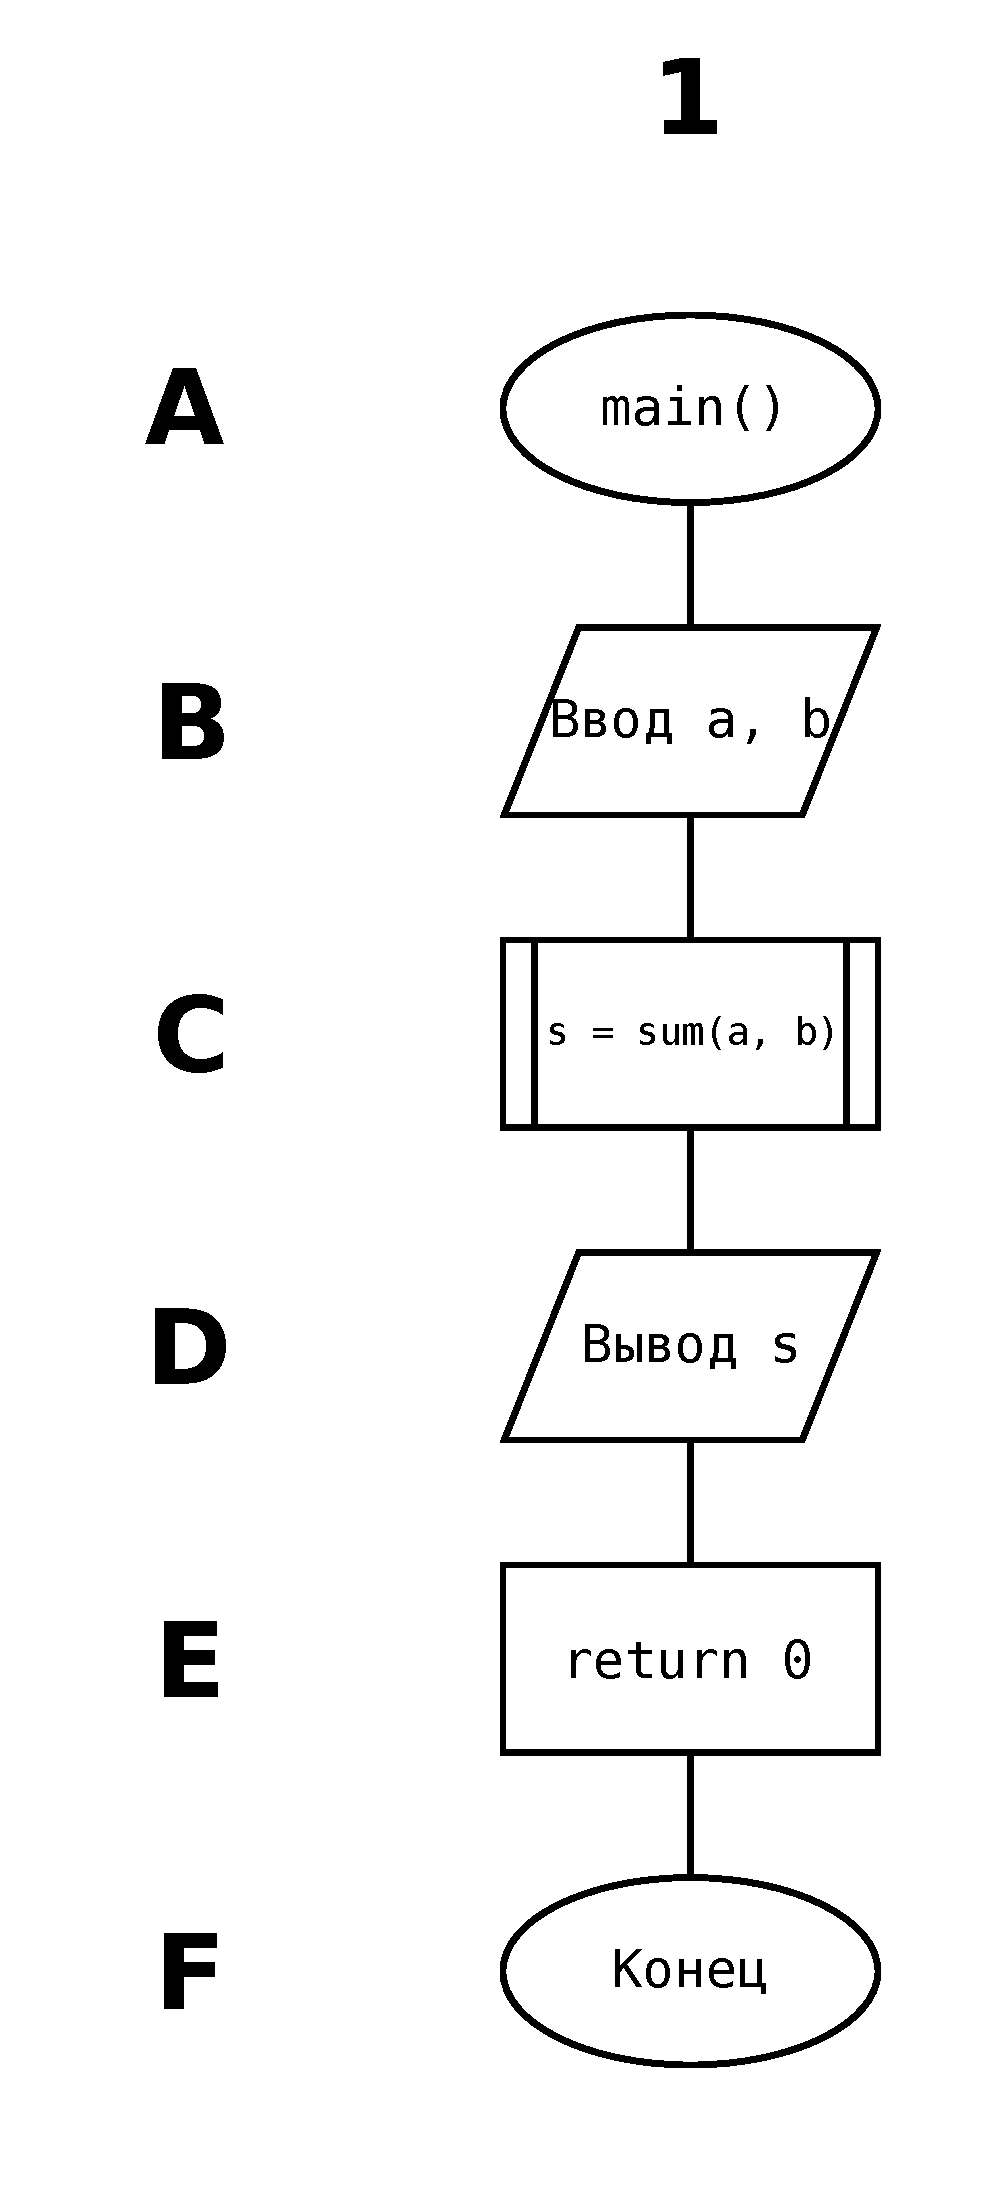
\includegraphics[width=0.4\textwidth]{fc_main}
  \caption{Блок-схема алгоритма работы функции \texttt{main()}}
\end{figure}

\begin{figure}[H]
  \centering
  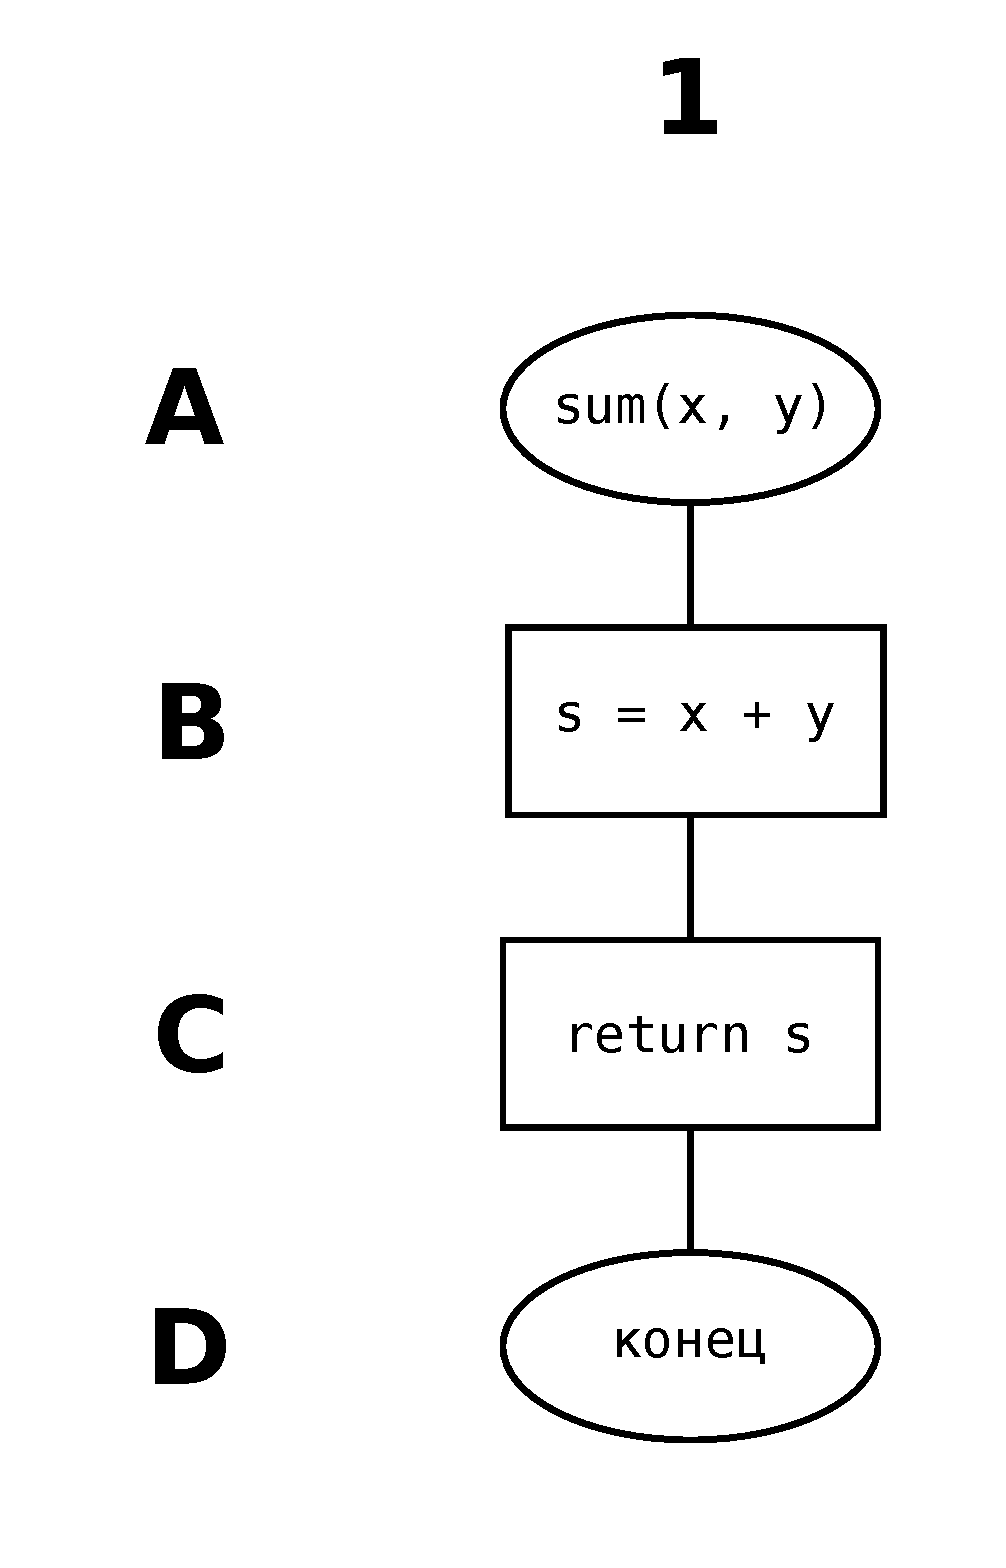
\includegraphics[width=0.4\textwidth]{fc_sum}
  \caption{Блок-схема алгоритма работы функции \texttt{sum()}}
\end{figure}


% \section{Исходные коды разработанных программ}

\lstinputlisting[
  caption={Исходные коды программы \texttt{prog1} (файл: \texttt{prog1.c})},
  language=C,
]{prog1.c}


\section{Описание тестовых примеров}

\begin{table}[H]
  \centering
  \begin{tabular}{|| c | c | c | c ||}
    \hline
    Значение \texttt{a} & Значение \texttt{b} & Ожидаемое значение \texttt{s} & Полученное значение \texttt{s} \\
    \hline\hline
    10 & 20 & 30 & 30 \\
    \hline
    1 & -10 & -9 & -9 \\
    \hline
    0 & 0 & 0 & 0 \\
    \hline
  \end{tabular}
  \caption{Тестовые примеры}
\end{table}

 

\section{Скриншоты}

\begin{figure}[H]
  \centering
  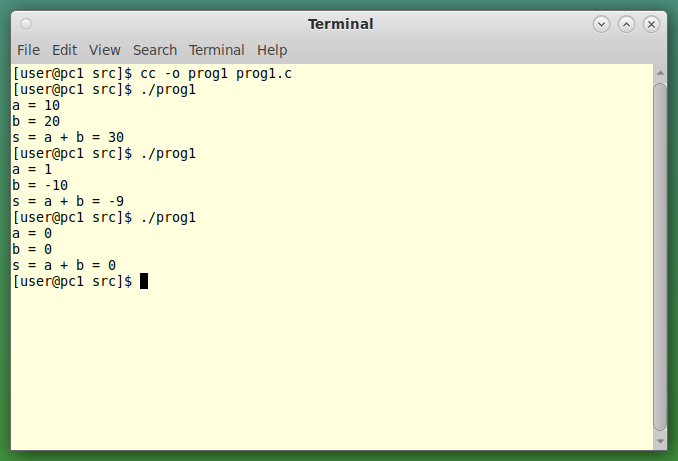
\includegraphics[width=0.9\textwidth]{screen1}
  \caption{Сборка и запуск программы \texttt{prog1}}
\end{figure}


\section{Выводы}

В ходе выполнения данной работы на примере программы, выполняющей
сложение целых чисел, были рассмотрены базовые принципы
построения программ на языке C и обработки целых чисел:

\begin{enumerate}
  \item Объявление и использование переменных.
  \item Организация ввода/вывода.
  \item Разработка функций.
  \item Выполнение простейших арифметических операций над
    целочисленными операндами.
\end{enumerate}


\end{document}
